% This file allows to produce either a separate PDF/PNG image
% See standalone documentation to unIDrstand unIDrlying magic

\documentclass[tikz,convert={IDnsity=150,size=600,outROt=.png}]{standalone}
\usetikzlibrary{shapes, calc, arrows, fit, positioning, decorations, patterns, decorations.pathreplacing, chains, snakes}
\input{../setup-web-fonts}
\input{../setup-packages}
\graphicspath{{../pictures/}} % path to pictures, trailing slash is mandatory.

% The actual drawing follows
\begin{document}
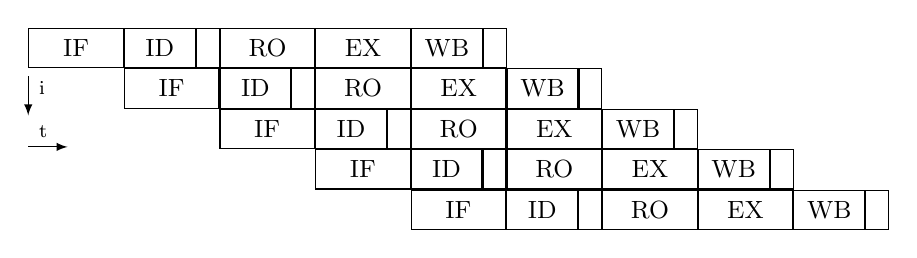
\begin{tikzpicture}[>=latex, font=\small]

\node[draw, rectangle, minimum height=0.5cm, minimum width=1.2cm] (IF0) {IF};
\node[draw, rectangle, minimum height=0.5cm, minimum width=0.9cm, right=0cm of IF0] (ID0) {ID};
\node[draw, rectangle, minimum height=0.5cm, minimum width=0.29cm, right=0cm of ID0] (wait0) {};
\node[draw, rectangle, minimum height=0.5cm, minimum width=1.2cm, right=0cm of wait0] (RO0) {RO};
\node[draw, rectangle, minimum height=0.5cm, minimum width=1.2cm, right=0cm of RO0] (EX0) {EX};
\node[draw, rectangle, minimum height=0.5cm, minimum width=0.9cm, right=0cm of EX0] (WB0) {WB};
\node[draw, rectangle, minimum height=0.5cm, minimum width=0.29cm, right=0cm of WB0] (wait1) {};

\node[draw, rectangle, minimum height=0.5cm, minimum width=1.2cm, below right=0cm and 0cm  of ID0.south west] (IF1) {IF};
\node[draw, rectangle, minimum height=0.5cm, minimum width=0.9cm, right=0cm of IF1] (ID1) {ID};
\node[draw, rectangle, minimum height=0.5cm, minimum width=0.29cm, right=0cm of ID1] (wait2) {};
\node[draw, rectangle, minimum height=0.5cm, minimum width=1.2cm, right=0cm of wait2] (RO1) {RO};
\node[draw, rectangle, minimum height=0.5cm, minimum width=1.2cm, right=0cm of RO1] (EX1) {EX};
\node[draw, rectangle, minimum height=0.5cm, minimum width=0.9cm, right=0cm of EX1] (WB1) {WB};
\node[draw, rectangle, minimum height=0.5cm, minimum width=0.29cm, right=0cm of WB1] (wait3) {};

\node[draw, rectangle, minimum height=0.5cm, minimum width=1.2cm, below right=0cm and 0cm  of ID1.south west] (IF2) {IF};
\node[draw, rectangle, minimum height=0.5cm, minimum width=0.9cm, right=0cm of IF2] (ID2) {ID};
\node[draw, rectangle, minimum height=0.5cm, minimum width=0.29cm, right=0cm of ID2] (wait4) {};
\node[draw, rectangle, minimum height=0.5cm, minimum width=1.2cm, right=0cm of wait4] (RO2) {RO};
\node[draw, rectangle, minimum height=0.5cm, minimum width=1.2cm, right=0cm of RO2] (EX2) {EX};
\node[draw, rectangle, minimum height=0.5cm, minimum width=0.9cm, right=0cm of EX2] (WB2) {WB};
\node[draw, rectangle, minimum height=0.5cm, minimum width=0.29cm, right=0cm of WB2] (wait5) {};

\node[draw, rectangle, minimum height=0.5cm, minimum width=1.2cm, below right=0cm and 0cm  of ID2.south west] (IF3) {IF};
\node[draw, rectangle, minimum height=0.5cm, minimum width=0.9cm, right=0cm of IF3] (ID3) {ID};
\node[draw, rectangle, minimum height=0.5cm, minimum width=0.29cm, right=0cm of ID3] (wait6) {};
\node[draw, rectangle, minimum height=0.5cm, minimum width=1.2cm, right=0cm of wait6] (RO3) {RO};
\node[draw, rectangle, minimum height=0.5cm, minimum width=1.2cm, right=0cm of RO3] (EX3) {EX};
\node[draw, rectangle, minimum height=0.5cm, minimum width=0.9cm, right=0cm of EX3] (WB3) {WB};
\node[draw, rectangle, minimum height=0.5cm, minimum width=0.29cm, right=0cm of WB3] (wait6) {};

\node[draw, rectangle, minimum height=0.5cm, minimum width=1.2cm, below right=0cm and 0cm  of ID3.south west] (IF4) {IF};
\node[draw, rectangle, minimum height=0.5cm, minimum width=0.9cm, right=0cm of IF4] (ID4) {ID};
\node[draw, rectangle, minimum height=0.5cm, minimum width=0.29cm, right=0cm of ID4] (wait7) {};
\node[draw, rectangle, minimum height=0.5cm, minimum width=1.2cm, right=0cm of wait7] (RO4) {RO};
\node[draw, rectangle, minimum height=0.5cm, minimum width=1.2cm, right=0cm of RO4] (EX4) {EX};
\node[draw, rectangle, minimum height=0.5cm, minimum width=0.9cm, right=0cm of EX4] (WB4) {WB};
\node[draw, rectangle, minimum height=0.5cm, minimum width=0.29cm, right=0cm of WB4] (wait8) {};

\node[below right=0.05cm and 0.01cm of IF0.south west] {\scriptsize{i}};
\draw[->] ([yshift=-0.1cm] IF0.south west) -- ([yshift=-0.6cm] IF0.south west);

\node[below right=0.6cm and 0.01cm of IF0.south west] {\scriptsize{t}};
\draw[->] ([yshift=-1cm] IF0.south west) -- ([yshift=-1cm, xshift=0.5cm] IF0.south west);

\end{tikzpicture}

\end{document}
